\documentclass{article}
\usepackage[utf8]{vietnam}
\usepackage{graphicx}    % needed for including graphics e.g. EPS, PS
\usepackage{listings}
\usepackage{tikz}
\usetikzlibrary{calc}
\usepackage{tikz-cd}
\usetikzlibrary{positioning}
\usetikzlibrary{decorations.markings}
\usepackage{xifthen}
\usetikzlibrary{shapes.geometric}
\tikzset{main node/.style={rectangle,fill=white,draw,minimum size=1cm,inner sep=0pt},}
\tikzset{black node/.style={circle,fill=black,draw,minimum size=0.4cm,inner sep=0pt},}
\usepackage{color}
\usepackage{amsthm}
\usepackage{verbatim}
\usepackage{caption}
\usepackage{amssymb}
\usepackage{fullpage}
\usepackage{mathrsfs}
\usepackage{epstopdf}
\usepackage{framed,color}
\usepackage[top=1in, bottom=1in, left=1in, right=1in]{geometry}
\usepackage{float}
\linespread{1.3}
\restylefloat{table}
\usepackage[tikz]{bclogo}
\usepackage{wrapfig}
\usepackage[intlimits]{mathtools}
\usepackage{indentfirst}
\usepackage{mdframed}
\usepackage{commath}
\usepackage{soul}
\usepackage{enumerate}
\usepackage{mathabx}
\definecolor{dkgreen}{rgb}{0,0.6,0}
\definecolor{gray}{rgb}{0.5,0.5,0.5}
\definecolor{mauve}{rgb}{0.58,0,0.82}
\definecolor{shadecolor}{rgb}{1,0.8,0.3}
\topmargin -1.5cm
\oddsidemargin -0.04cm
\evensidemargin -0.04cm
\textwidth 16.59cm
\textheight 24cm
\parskip 7.2pt
\parindent 15pt
\DeclareMathOperator*{\esssup}{ess\,sup}
\newcommand*{\bigchi}{\mbox{\Large$\chi$}}% big chi
\newtheorem{vtheorem}{Định lý}
\newtheorem{vcorollary}{Hệ quả}
\newtheorem{vlemma}{Bổ đề}
\newtheorem{vproposition}{Tính chất}
\renewcommand*{\proofname}{Chứng minh}
\newtheorem*{vnote}{Ghi chú}

\title{Notes 2 tháng 7}
\author{Nguyễn Nga Nhi}

\begin{document}

\maketitle

\section{Machine Learning}

Mô hình tổng quát: TEFPA

+ T = Task

+ E = Experience

+ F = Function

+ P = Performance

+ A = Algorithm

Machine Learning Framework: Simplfied + Unified

+ Simplified = đơn giản hóa

+ Unified = đa dạng input

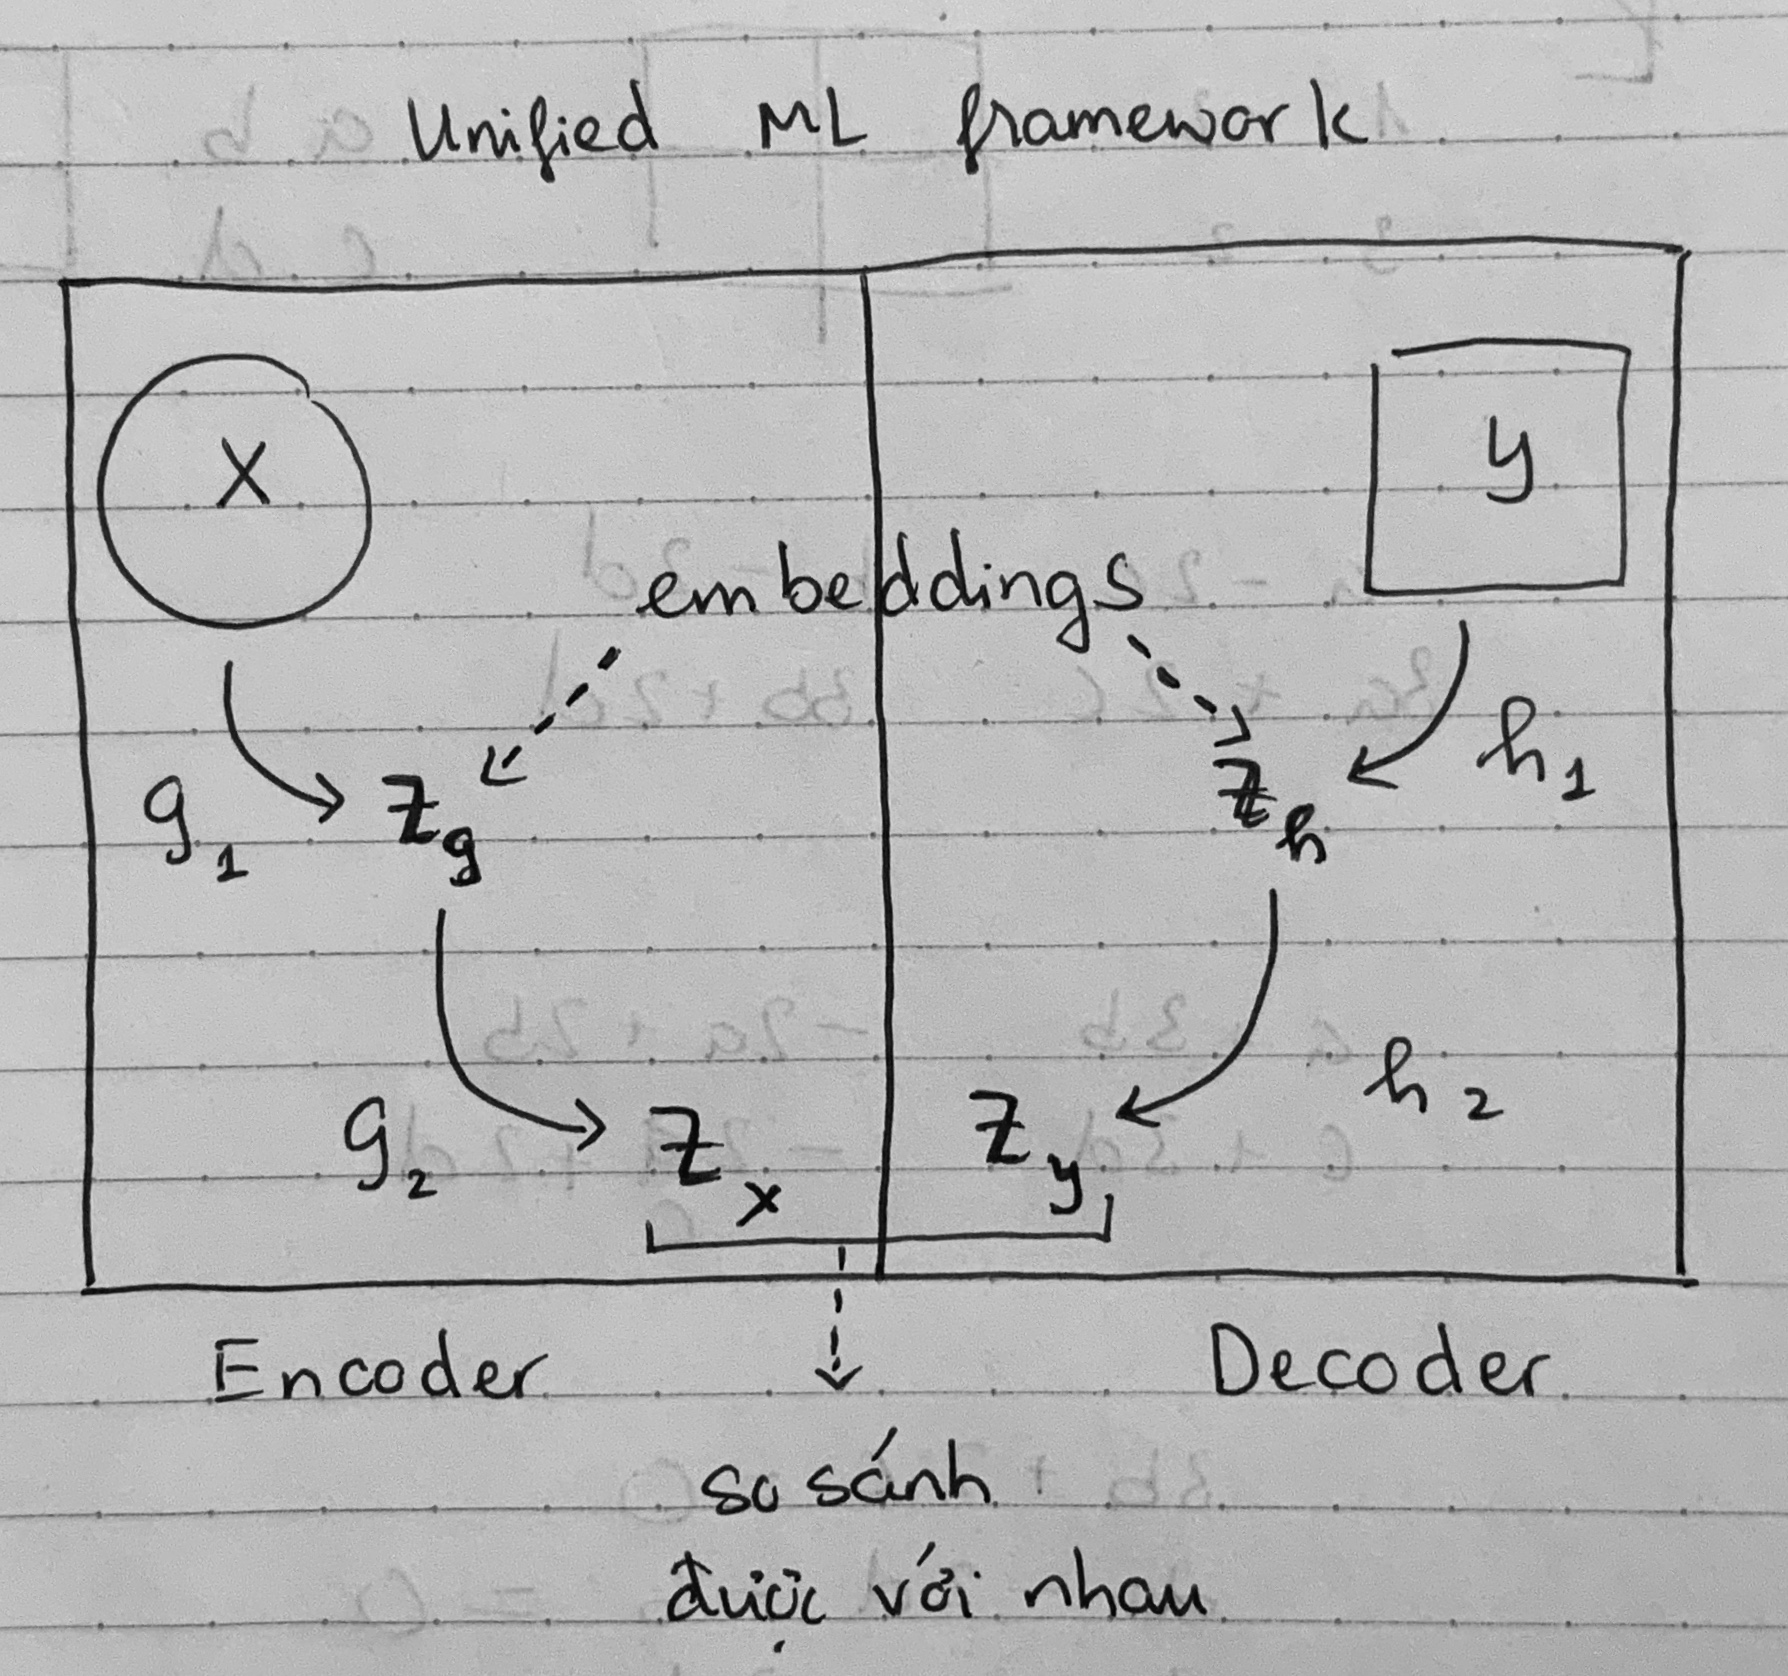
\includegraphics[width=230]{Unified ML Framework.jpg}

+ X = data

+ Y = label

+ $g_1$, $h_1$ = hàm trích xuất

+ $Z_g$, $Z_h$ = embedding / vector coordinate

+ $Z_x$, $Z_y$ = thành phần tương ứng có thể so sánh

+ $g_2$, $h_2$ = thuật toán sao cho $Z_x$, $Z_y$ gần nhau nhất

\section{Basis functions}

Hàm đặc trưng: Trích xuất đặc trưng của input

+ output: vector coordinate Z 

(1 basis $\implies$ 1 axis $\implies$ 1 coordinate)

\section{Principle Component Analysis}

PCA

Giảm chiều dữ liệu: Lựa chọn k thành phần chính

Biểu diễn:

$$X = X_0 + z_1 X_1 + z_2 X_2 + \dots + z_k X_k$$


+ $X_0$ = TBC \space training \space data

+ $X_i$ = basis function

+ $z_i$ = coordinate

So sánh khác biệt giữa 2 vector $X_1, X_2$

+ khoảng cách = $\sqrt{\sum (x_{1_{ij}} - x_{2_{ij}})^2}$

+ góc = $\sqrt{\sum x_{1_{ij}} x_{2_{ij}}}$

\end{document}
